\documentclass{homeworg}
\usepackage{threeparttable}
\usepackage{lscape}
\usepackage{natbib}
\usepackage{amsmath}
\usepackage{graphicx}
\usepackage{listings}
\usepackage{booktabs}
\usepackage{caption}
\usepackage{subcaption}


\title{Bayesian Statistics Midterm}
\author{Weijia Zhao}



\begin{document}
\maketitle

\textbf{Caution:}
\begin{itemize}
\item  I keep 6 digits for all decimal numbers. For simulated results, since it involves random sampling from
certain non-degenerative distribution, the results may be slightly different in different trials (and thus from the official solution)
\item There is some ambiguity in Q3, see detailed explanation page 4

\end{itemize}

\exercise 
\textbf{Quality Control} \\
10 products were inspected and none of them were rejected

(a) Assume the prior distribution of rejecting a product , $\theta$ is $U(0,1)$, denote these observations by $\{x_i\}_{i=1}^{10}$, then the posterior distribution is given by 
\begin{align*}
\pi(\theta|\{x_i\}_{i=1}^{10})& \propto \pi(\theta)*\Pi_{i=1}^{10}f(x_i| \theta)\\
&=1*(1-\theta)^{10}
\end{align*}
To find the normalizing constant, we integrate the expression and get 
\begin{align*}
\int_{0}^{1} (1-\theta)^{10} d\theta &= \frac{1}{11}
\end{align*}
So the posterior distribution is given by

$$ \pi(\theta|\{x_i\}_{i=1}^{10})=\left\{
\begin{aligned}
11(1-\theta)^{10} &, & 0 \leq \theta \leq 1\\
0 &,& \text{else}
\end{aligned}
\right.
$$

Thus the posterior mean is given by $\int_{0}^{1}\pi(\theta|\{x_i\}_{i=1}^{10}) *\theta d\theta=\frac{1}{12}$ (Actually the posterior distribution is a special case of $Beta$ distribution $Beta(\alpha=1,\beta=11)$ if we look closely at its kernel $(1-\theta)^{10}$, we can directly apply the mean of $Beta$ distribution $\frac{\alpha}{\alpha+\beta}=\frac{1}{12}$)

(b) For the $(1-\alpha)$ equitailed credible interval, we need to find $\theta_L$ and $\theta_H$ such that 
\begin{align*}
\frac{\alpha}{2}&=\int_{0}^{\theta_L}11(1-\theta)^{10}d\theta =(\theta-1)^{11}|_{0}^{\theta_L}=(\theta_L-1)^{11}-(-1)^{11}=(\theta_L-1)^{11}+1\\
\frac{\alpha}{2}&=\int_{\theta_H}^{1}11(1-\theta)^{10}d\theta=(\theta-1)^{11}|_{\theta_H}^1=0^{11}-(\theta_H-1)^{11}=-(\theta_H-1)^{11}
\end{align*}
Solve the two equations listed above, we have $\theta_L=1-(1-\frac{\alpha}{2})^{\frac{1}{11}}$ and $\theta_H=1-(\frac{\alpha}{2})^{\frac{1}{11}}$, thus the $(1-\alpha)$ equitailed credible interval is given by $[1-(1-\frac{\alpha}{2})^{\frac{1}{11}}, 1-(\frac{\alpha}{2})^{\frac{1}{11}}]$

(c) For the $(1-\alpha)$ HPD credible interval, notice that the posterior distribution is strictly decreasing over it domain $0\leq \theta \leq 1$, thus we need to find $\theta_L$ and $\theta_H$ such that 
\begin{align*}
0&=\theta_L\\
\alpha&=\int_{\theta_H}^{1}11(1-\theta)^{10}d\theta=(\theta-1)^{11}|_{\theta_H}^1=0^{11}-(\theta_H-1)^{11}=-(\theta_H-1)^{11}
\end{align*}
Solve the two equations listed above, we have $\theta_L=0$ and $\theta_H=1-\alpha^{\frac{1}{11}}$, thus the $(1-\alpha)$ HPD credible interval is given by $[0,1-\alpha^{\frac{1}{11}}]$

\exercise 
\textbf{Waiting Time} \\
Waiting time for a bus has a $U(0,\theta)$ distribution and want to test $H_0: 0\leq\theta\leq 15$ v.s. $H_1: \theta>15$, $\theta$ has a prior $Pareto(5,3)$ where $Pareto(\xi,\gamma)$ has density $p(x;\xi,\gamma)=
\frac{\gamma\xi^\gamma}{x^{\gamma+1}}\mathbb{I}_{(\xi,\infty)}(x)$. Observations are 10, 3, 2, 5, 14. 

We know that the prior distribution of $\theta$ is given by 
\begin{align*}
\pi(\theta)=\frac{3*5^3}{\theta^{3+1}}\mathbb{I}_{(5,\infty)}(\theta)=
\frac{375}{\theta^4}\mathbb{I}_{(5,\infty)}(\theta)
\end{align*}
Denote the observations by $\{x_i\}_{i=1}^5$, notice that the domain of observations is $[0,\theta]$,  we have $\theta\geq x_i, \forall x_i$, we have the posterior distribution given by 
\begin{align*}
p(\theta|\{x_i\}_{i=1}^5)&\propto \pi(\theta)*\Pi_{i=1}^5f(x_i|\theta)\\
&=\frac{375}{\theta^4}\mathbb{I}_{(5,\infty)}(\theta)*\Pi_{i=1}^5(\frac{1}{\theta}\mathbb{I}_{\theta>x_i})\\
&=\frac{375}{\theta^9}\mathbb{I}_{(5,\infty)}(\theta)*\mathbb{I}_{(10,\infty)}(\theta)*\mathbb{I}_{(3,\infty)}(\theta)*\mathbb{I}_{(2,\infty)}(\theta)*\mathbb{I}_{(5,\infty)}(\theta)*\mathbb{I}_{(14,\infty)}(\theta)\\
&=\frac{375}{\theta^9}*\mathbb{I}_{(14,\infty)}(\theta)
\end{align*}
This is still a kernel of the Pareto distribution and the parameters are given by $\gamma+1=9$, $\xi=14$, i.e. $\gamma=8$, $\xi=14$, thus the posterior distribution is given by 
\begin{align*}
p(\theta|\{x_i\}_{i=1}^5)=\frac{8*14^8}{\theta^9}\mathbb{I}_{(14,\infty)}(\theta)
\end{align*}
The posterior odds is given by 
\begin{align*}
\frac{p_0}{p_1}=\frac{\int_{0}^{15}\frac{8*14^8}{\theta^9}\mathbb{I}_{(14,\infty)}(\theta)d\theta}{\int_{15}^{\infty}\frac{8*14^8}{\theta^9}\mathbb{I}_{(14,\infty)}(\theta)d\theta}=0.736624
\end{align*}
Recall that the prior odds is given by 
\begin{align*}
\frac{\pi_0}{\pi_1}=\frac{\int_{0}^{15}\frac{375}{\theta^4}\mathbb{I}_{5,\infty}(\theta)d\theta}{\int_{15}^{\infty}\frac{375}{\theta^4}\mathbb{I}_{(5,\infty)}(\theta)d\theta}=26
\end{align*}
Thus the Bayes factor in favor of $H_0$ is given by $B_{01}=\frac{p_0/p_1}{\pi_0/\pi_1}=\frac{0.736624}{26}$ and the Bayes factor against $H_0$ is given by $B_{10}=\frac{26}{0.736624}=35.296164$, since $\log_{10}B_{10}=1.547728$, we have very strong evidence against $H_0$

\exercise 
\textbf{Casting Defects} \\
Number of defects follow Poisson distribution with mean $\theta$, the density is given by $\frac{\theta^ke^{-\theta}}{k!}$. Observations are 0,2,2,3,3,1,2,1,1. $\theta$ has a prior distribution $Gamma(2,b)$ where density of $Gamma(a,b)$ is $\frac{b^a\theta^{a-1}e^{-b\theta}}{\Gamma(a)}$. The hyperparameter b has a distribution $Exp(1)$ where the density of $Exp(\lambda)$ is $\lambda e^{-\lambda b}$

As the prior distribution of $\theta$ is given by $\frac{b^2x^1e^{-bx}}{\Gamma(2)}$, denote the observations by $\{x_i\}_{i=1}^9$ (the number/frequency of value 0 is 1, the number/frequency of value 1 is 3, the number/frequency of value 2 is 3, the number/frequency of value 3 is 2), we have the joint distribution of $\theta,b$ given by 
\begin{align*}
f(\theta,b,\{x_i\}_{i=1}^n)&\propto f(b)\pi(\theta|b)*\Pi_{i=1}^9f(x_i|\theta)\\
&=\lambda e^{-\lambda b} \frac{b^2\theta ^1e^{-b\theta}}{\Gamma(2)}*\Pi_{i=1}^9(\frac{\theta^{x_i}e^{-\theta}}{x_i!})\\
&=\lambda e^{-\lambda b}\frac{b^2\theta ^1e^{-b\theta}}{\Gamma(2)}*(\frac{\theta^{0}e^{-\theta}}{0!})*(\frac{\theta^{1}e^{-\theta}}{1!})^3*(\frac{\theta^{2}e^{-\theta}}{2!})^3*(\frac{\theta^{3}e^{-\theta}}{3!})^2\\
&=\lambda e^{-\lambda b}\frac{b^2\theta^{1+0+1*3+2*3+3*2}e^{-\theta(b+1+1*3+1*3+1*2)}}{\Gamma(2)*1*1^3*2^3*6^2}\\
&=\lambda e^{-\lambda b}\frac{b^2*\theta^{16}e^{-\theta(b+9)}}{\Gamma(2)*288}\\
&=\frac{\lambda b^2}{\Gamma(2)*288} \theta^{16}e^{-\theta(b+9)-\lambda b}\\
&\propto b^2 \theta^{16}e^{-\theta(b+9)-\lambda b}
\end{align*}

For the posterior distribution of $\theta|(b,\{x_i\}_{i=1}^n)$, we only focus on the term with $\theta$, which is $\theta^{16}e^{-\theta(b+9)}$, this is the kernel of $Gamma(17,b+9)$ (i.e. $Gamma(2+\sum_{i=1}^{n}x_i,b+n)$, where n is the number of observations). 

\textbf{Notice that there is some ambiguity in the question whether we should treat the distribution of $b\sim Exp(1)$ as a prior distribution or as something we are already sure about/there is no uncertainty about it (i.e. whether the distribution of $b$ is updatable or not).} I include both cases below though the first case seems to be more aligned with the example questions in lecture notes (but the lecture note is explicit that a certain distribution is a \textbf{prior})

\begin{itemize}
\item In the first case, we treat $b\sim Exp(1)$ as a prior distribution, then the posterior distribution of $b$ is given by only focusing on terms with b, that is $b|(\theta,\{x_i\}_{i=1}^n)\sim b^2e^{-(\theta+\lambda)b}$, which is the kernel of $Gamma(3,\theta+\lambda)=Gamma(3,\theta+1)$ as $\lambda=1$
\item In the second case, we treat $b\sim Exp(1)$ as something fixed and not updatable, then we still sample $b$ from $Exp(1)$
\end{itemize}

For the first case, the Gibbs sampling is given by the following steps
\begin{itemize}
	\item Initialize $\theta_0$
	\item Sample b from $Gamma(3,\theta+1)$
	\item Sample $\theta$ from $Gamma(17,b+9)$
	\item With the newly obtained $\theta$, go back to step (2), repeat the steps (2) and (3) above until we get enough observations (ignore the first 1000 observations)
\end{itemize}

For the second case, the Gibbs sampling is given by the following steps\footnote{Note that this is actually a degenerated Gibbs sampler as we only have one way dependence in the distributional assumption (i.e. $\theta$ is dependent on b but not the other way around)}
\begin{itemize}
\item Sample b from $Exp(1)$
\item Sample $\theta$ from $Gamma(17,b+9)$
\item Repeat the two steps above until we get enough observations (ignore the first 1000 observations)
\end{itemize}


(a) See the following graph
\begin{figure}[h]
	\centering
	\begin{subfigure}[b]{0.48\textwidth}
		\centering
		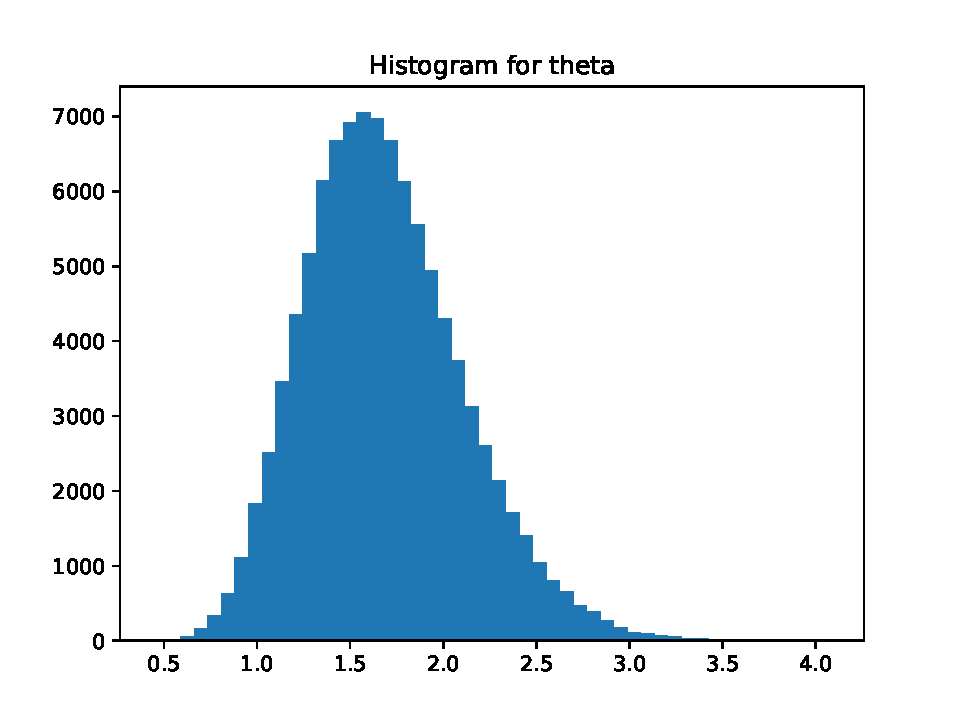
\includegraphics[width=\textwidth]{q3_parta_hist_theta_case1.pdf}
		\caption{Case 1: When distribution of $b$ is a prior (updatable)}
	\end{subfigure}
	\hfill
	\begin{subfigure}[b]{0.48\textwidth}
		\centering
		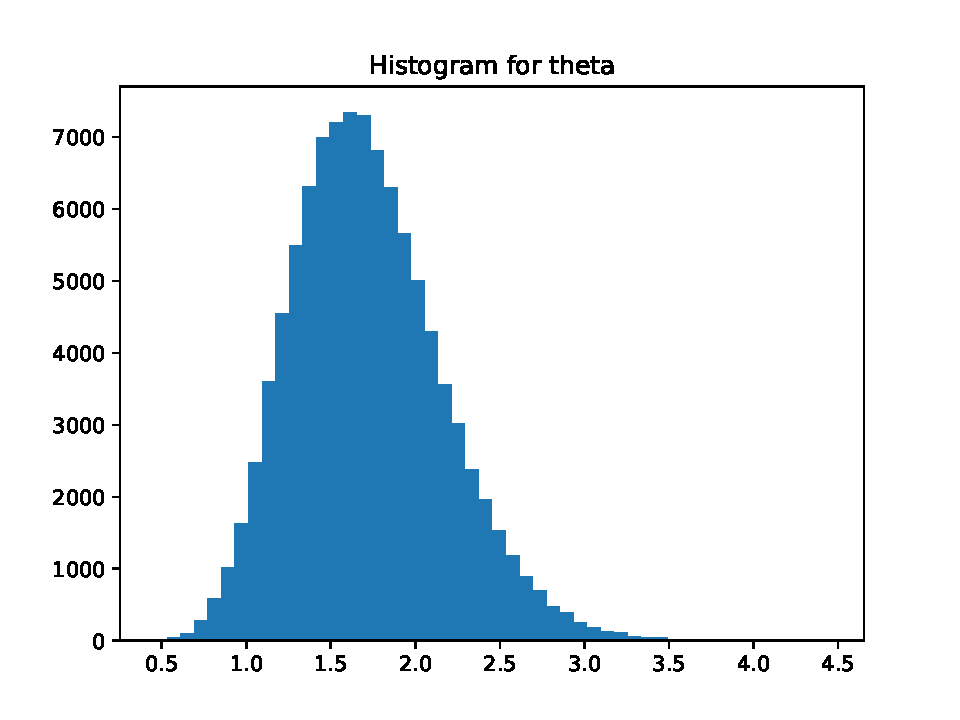
\includegraphics[width=\textwidth]{q3_parta_hist_theta_case2.pdf}
		\caption{Case 2: When distribution of $b$ is fixed (not updatable)}
	\end{subfigure}
	\caption{Histogram of $\theta$}
\end{figure}
Notice that for this question and the questions below, the results for both cases are very close mainly because the posterior distribution of $b$ does not really shift too much from its prior.

(b) 
\begin{itemize}
\item In case 1: The posterior mean of $\theta$ is given by 1.683211 when we assume the distribution of $b\sim Exp(1)$ is a prior distribution and we update it along the way. The posterior mean of $b$ is 1.142747
\item In case 2: 1.717011 when we assume the distribution of $b\sim Exp(1)$ is a distribution that we already know and we fix it, not update it along the way. The mean of $b$ is 0.995968
\end{itemize}


(c) 
\begin{itemize}
\item Case 1: The 95\% equitailed credible interval is given by (0.961401, 2.616482) when we assume the distribution of $b\sim Exp(1)$ is a prior distribution and we update it along the way
\item Case 2: The 95\% equitailed credible interval is given by (0.957683, 2.690481) when we assume the distribution of $b\sim Exp(1)$ is a distribution that we already know and we fix it, not update it along the way
\end{itemize} 



%\setlength\bibsep{0pt}
%\bibliographystyle{apalike}
%\bibliography{hw1}

\pagebreak
\lstinputlisting[language=Python]{q3.py}
%\include{q3.py}
%\lstinputlisting[]{Untitled.do}

\end{document}








